\documentclass[11pt]{article}

\usepackage[catalan]{babel}
\usepackage[utf8]{inputenc}
\usepackage[T1]{fontenc}
\usepackage{lmodern}
\usepackage{multirow}
\usepackage{graphicx}
\usepackage[a4paper,total={6.4in,9.5in}]{geometry}
\usepackage{pdflscape}
% Formatting options
\usepackage[bf,sf]{titlesec} % Make the section titles bold and sans-serif
\usepackage[font={footnotesize, sf}, labelfont=bf]{caption} % Format dels peus de figura
\renewcommand{\arraystretch}{1.7}
\usepackage{amsmath,amssymb}
\usepackage{amsmath}

\newcommand{\abs}[1]{\left\lvert#1\right\rvert}
\newcommand{\R}{\mathbb{R}}
\newcommand{\N}{\mathbb{N}}

\newcommand{\yestag}{\refstepcounter{equation}\tag{\theequation}}

\title{\sffamily {\bfseries EDIM I:} Informe calefacció}
\author{\sffamily Raquel García Bellés, Miquel Saucedo Cuesta}
\date{}

\begin{document}
	
\maketitle
\section*{Introducció i supòsits}
Se'ns demana pensar diversos models pel funcionament del temporitzador de la calefacció d'un habitatge. Així doncs, caldrà tenir en compte factors com l'horari de les persones que hi viuen, el rang de temperatures que es considera "agradable", i la despesa energètica. \\

 

L'evolució temporal de la temperatura vindrà donada per l'equació diferencial:
\begin{equation}\label{principal}
	T'=q(t)-k(T-T_e(t)),\quad T(t_0)=T_0
\end{equation}
on $T$ és la temperatura a l'interior, $T_e(t)$ és la temperatura exterior, $q(t)$ és la funció que quantifica l'acció de la calefacció, i $k$ és una constant que mesura el ritme al qual s'intercanvia calor amb l'exterior, i que depèn, entre d'altres coses, de característiques de l'habitatge com la geometria i l'aïllament tèrmic. Aquesta constant pot determinar-se empíricament si es disposa dels valors de la temperatura exterior i interior de l'habitatge per a diferents temps. En el nostre model prendrem $k=0.1$, ja que fent assajos amb $q(t)=0$, aquest valor ens donava un ritme raonable\footnote{Amb la $T_e(t)$ definida en l'equació \eqref{te}, de les $23:00$h a les $24:00$h la temperatura baixa aproximadament $1$ºC.} d'intercanvi de calor.\\

Considerarem la temperatura de l'habitatge en el transcurs de 24 hores. En aquesta escala temporal, és una bona aproximació suposar que la temperatura exterior varia seguint una funció sinusoidal segons:
 \begin{equation}\label{te}
T_e(t)=\frac{T_{max}+T_{min}}{2}+\frac{T_{max}-T_{min}}{2}\sin\left(\omega t+\pi\right)
\end{equation}
Amb $T_{max}=15$ºC, $T_{min}=5$ºC i $\omega=2\pi/24$. Hem escollit aquestes temperatures per a simular la temperatura d'un dia d'hivern en una ciutat com Barcelona \cite{df}. El desfasament de $\pi$ s'ha introduït per tal que a les $6:00$h de la matinada es doni la temperatura mínima.\\

En cada model proposarem una $q(t)$, i valorarem la seua eficiència segons una estimació de la despesa energètica, $E$, que calcularem mitjançant:\\
\begin{equation}\label{gasto}
	E=\int^{t_0+24}_{t_0} q(t)dt
\end{equation}

Suposarem que l'horari en el qual hi ha gent a l'interior és de $17:00$h fins a $9:00$h del dia següent, de manera que hem fixat $q(t\in[9,16])=0$ en tots els models amb l'objectiu d'estalviar energia. A les 16:00h s'engegarà la calefacció per tal d'obtenir la temperatura desitjada a les 17:00h. També suposarem que els valors òptims de temperatura pels habitants estan entre $22$ i $23$ºC. A l'hora de resoldre l'equació diferèncial \eqref{principal}, prendrem com a condicions inicials $t_0=16$ i $T_0=T_e(t_0)$ en tots els models.\\
\section*{Models}
	\subsection{Model 1}
	Aquest model pretén imitar el funcionament d'un termòstat, de manera que quan la temperatura baixa de $23$ºC s'activa la calefacció. A més la calor subministrada és proporcional a la diferència entre la temperatura actual a l'interior i la desitjada.
	\subsubsection*{Model 1.1}
	En aquest model pretenem mantenir la temperatura entre $22$ i $23$ºC mentre hi hagi gent a l'interior. Per això definim:
	\begin{equation}\label{model11}
	 q(t\in[16,9+24])=
		\begin{cases}
		r(23-T)&\text{si}\quad T<23\\
		0&\text{si}\quad T\geq23
		
		\end{cases}
	\end{equation}
	on $r$ és un paràmetre que hem ajustat de manera que a les 17:00h la temperatura sigui superior a $22$ºC, i que fins a les 9:00h del dia següent sempre es mantingui per sobre d'aquesta temperatura. A més hem pres el valor que ens donava menor despesa energètica, aquest ha sigut $r=2.43$. Per simplicitat, hem resolt l'equació diferencial \eqref{principal} numèricament amb el métode de Runge-Kutta d'ordre 4, i hem  obtingut la despesa energètica d'aquest model integrant numèricament l'expressió \eqref{gasto}, aquesta ha estat de $E=29.30$. Els resultats obtinguts per a l'evolució de la temperatura amb aquest model, així com la funció $q(t)$ es representen en la figura \ref{figmodel11}. 
	\begin{figure}[h!]
		\centering
		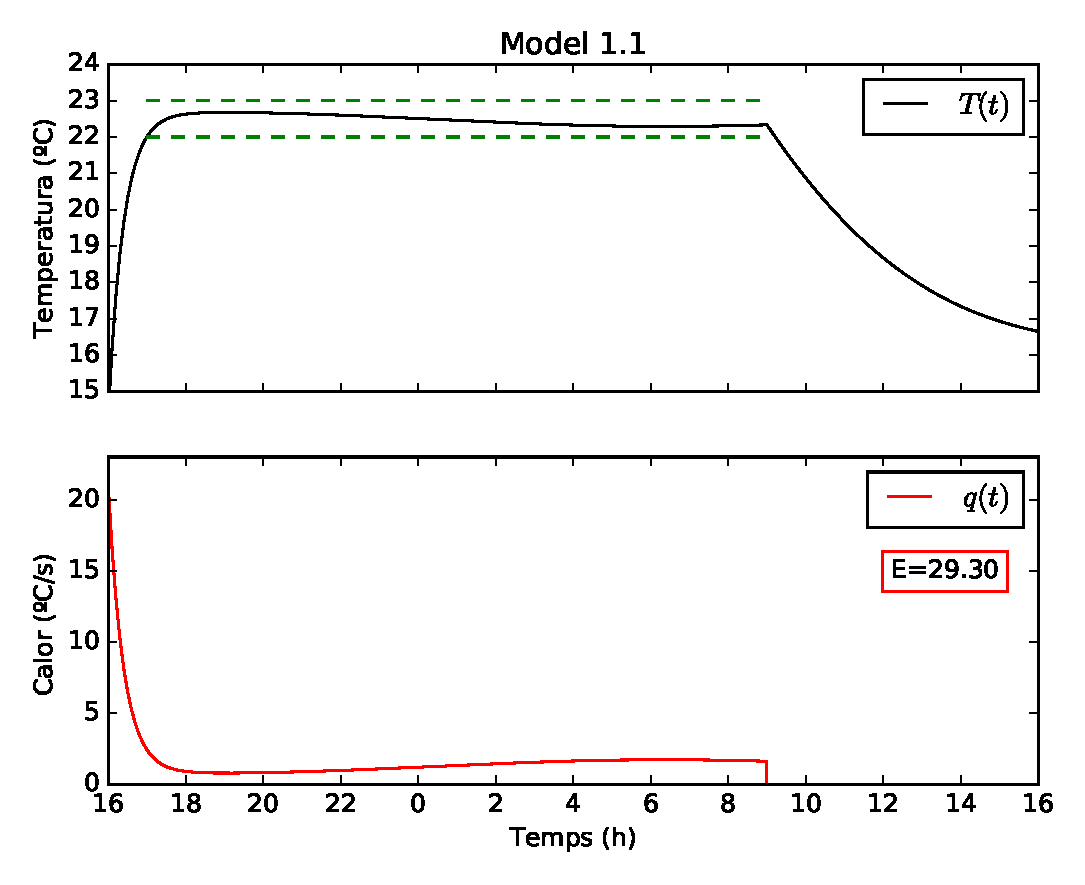
\includegraphics[width=12cm]{model11.eps}
		\caption{La gràfica superior mostra l'evolució de la temperatura a l'interior de l'habitatge en funció del temps. Les línies puntejades senyalen el rang de temperatures que es considera acceptable. La gràfica inferior mostra el comportament de $q(t)$. Observem que en cap moment s'han assolit els $23$ºC.}
		\label{figmodel11}
	\end{figure}
	\subsubsection*{Model 1.2}
	Aquest model és una variació de l'anterior, en el qual considerem que desde les 23:00h fins a les 7:00h els habitants estan dormint. És una pràctica habitual posar la calefacció més baixa per la nit per tal d'estalviar energia, tot i això tampoc es pot permetre que la temperatura baixi excesivament per a mantenir el comfort dels habitants. Així doncs, en aquesta franja horària la calefacció s'activarà quan la temperatura baixi de $18$ºC, i a les 6:00h tornarà a posar-se més forta per aconseguir que a les 7:00h la temperatura torni a ser de $22$ºC. Definim:
\begin{align} 
q(t\in[16,23])&=
\begin{cases}
r_1(23-T)&\text{si}\quad T<23\\
0&\text{si}\quad T\geq23
\end{cases}
\\
q(t\in[23,6+24])&=
\begin{cases}\label{caiguda}
r_2(18-T)&\text{si}\quad T<18\\
0&\text{si}\quad T\geq18
\end{cases}
\\
q(t\in[6+24,9+24])&=
\begin{cases}
r_3(23-T)&\text{si}\quad T<23\\
0&\text{si}\quad T\geq23
\end{cases}
\end{align}
on $r_1$, $r_2$ i $r_3$ són paràmetres. $r_1$ i $r_3$ s'han ajustat de manera que entre les 17:00h i les 23:00h, i entre les 7:00h i 9:00h del dia següent respectivament la temperatura sigui superior a $22$ºC. El paràmetre $r_3$ s'ha ajustat per no permetre que la temperatura baixi dels $17$ºC entre les 23:00h i les 6:00h del dia següent. Per a tots tres s'ha triat aquell valor que minimitzava la despesa energètica i aquests han sigut: $r_1=2.43$, $r_2=1.16$ i $r_3=2.64$. L'equació diferèncial s'ha resolt novament utilitzant el mètode Runge-Kutta d'ordre 4, i la despesa energètica integrant numèricament l'expressió \eqref{gasto}, aquesta ha estat de $E=27.22$. Els resultats obtinguts es representen en la figura \ref{figmodel12}.\\

	\begin{figure}[h!]
		\centering
		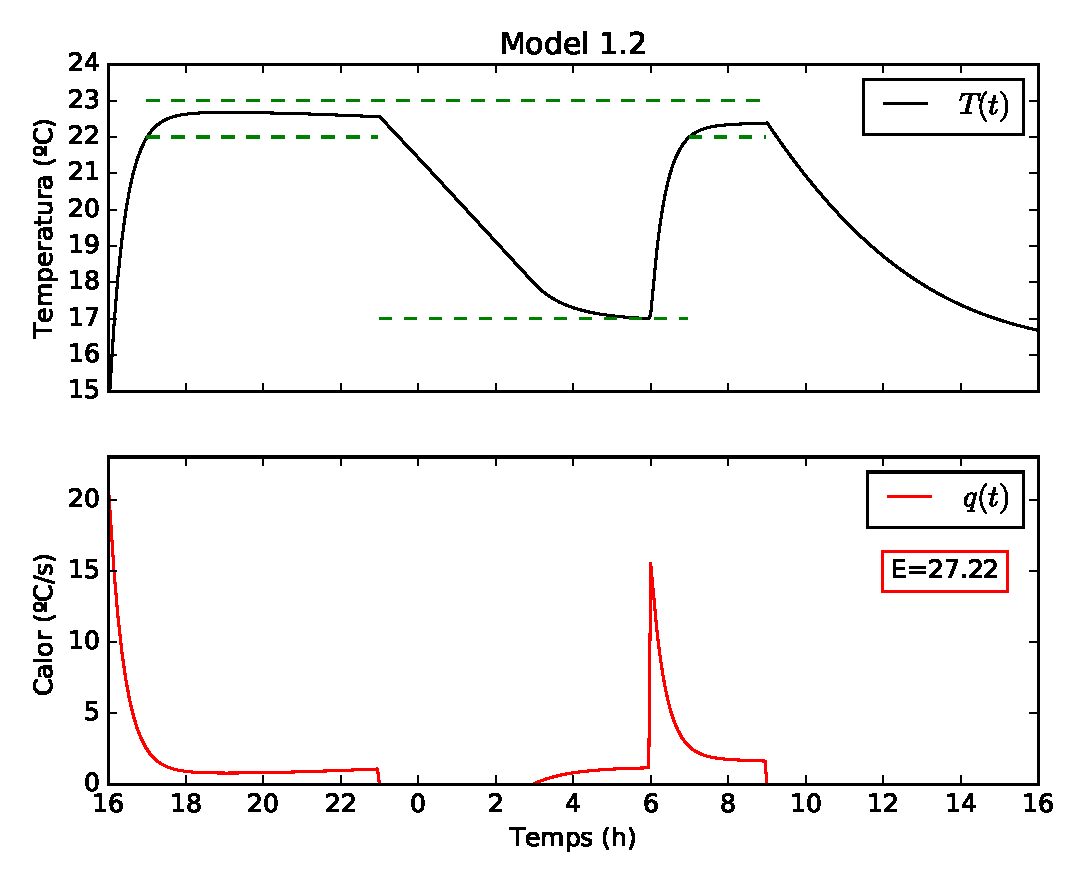
\includegraphics[width=12cm]{model12.eps}
		\caption{Evolució de la temperatura en funció del temps i $q(t)$ aplicada en el model 1.2. Observem com l'expressió \eqref{caiguda} suavitza la caiguda de temperatura durant la nit. També notem que ha hi hagut una disminució de la despesa energètica de més de 2 punts respecte al model 1.1.}
		\label{figmodel12}
	\end{figure}
	En els models posterior permetrem que entre les 23:00h i les 7:00h la temperatura estigui entre $17$ i $22$ºC per tal de reduir la despesa energètica.
	\section{Model 2}
	Observem que si tenim una funció:
	\begin{equation}\label{constant}
		f(t)=k(T-T_e(t))
	\end{equation}
	introduïnt \eqref{constant} com a $q(t)$ en \eqref{principal}, obtenim $T'=0$, per tant aquesta funció permet mantenir la temperatura constant. Així doncs considerem per a aquest model:
	\begin{align} 
	q(t\in[16,17])&=
	\begin{cases}
	r_1(23-T)&\text{si}\quad T<23\\
	0&\text{si}\quad T\geq23
	\end{cases}
	\\
	q(t\in[17,23])&=k(T-T_e(t))\\
	q(t\in[23,6+24])&=
	\begin{cases}
	k(T-T_e(t))&\text{si}\quad T\leq17\\
	0&\text{si}\quad T>17
	\end{cases}
	\\
		q(t\in[6+24,7+24])&=
		\begin{cases}
		r_2(23-T)&\text{si}\quad T<23\\
		0&\text{si}\quad T\geq23
		\end{cases}
		\\
	q(t\in[7+24,9+24])&=k(T-T_e(t))
	\end{align}
	$r_1$ i $r_2$ són paràmetres que s'han ajustat per tal d'obtenir una temperatura de $22$ºC a les 17:00h i a les 7:00h, si es comença a pujar la temperatura a les 16:00h i a les 6:00h respectivament, aquests valen: $r_1=2.43$ i $r_2=2.64$. L'equació diferencial \eqref{principal} s'ha resolt numèricament utilitzant el mètode Runge-Kutta d'ordre 4, i la despesa energètica s'ha calculat integrant numèricament l'expresió \eqref{gasto}, aquesta ha sigut $E=26.49$. En la figura \ref{figmodel2} és representen els resultats obtinguts.
	\begin{figure}[h!]
		\centering
		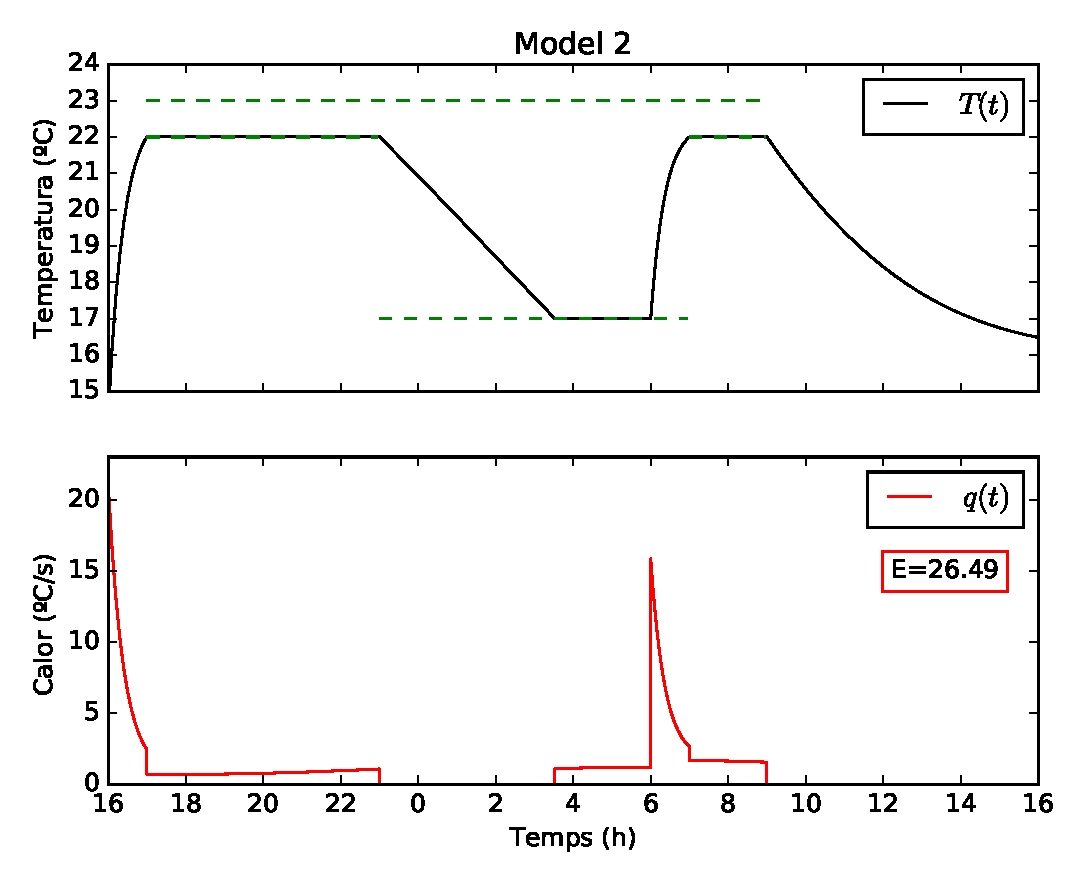
\includegraphics[width=12cm]{model2.eps}
		\caption{blabl}
		\label{figmodel2}
	\end{figure}
	\section{Model 3}
	Observem que si tenim una funció $f(t)$ que depén de com estigui variant la temperatura de la casa, segons:
	\begin{equation}\label{model2_1}
		f(t)=\alpha T'(t)
	\end{equation}
	on $\alpha$ és una constant. Aleshores al introduïr \eqref{model2_1} com a $q(t)$ en \eqref{principal} obtenim:
	\begin{equation}
		T'=-\frac{k}{1-\alpha}(T-T_e(t))
	\end{equation}
	de manera que si anomenem $k'=k/(1-\alpha)$, aquesta funció és equivalent a poder canviar la constant $k$. Així doncs, en aquest model considerem la següent $q(t)$:
	\begin{align} 
	q(t\in[16,17])&=
	\begin{cases}\label{pujar1}
	r_1(23-T)&\text{si}\quad T<23\\
	0&\text{si}\quad T\geq23
	\end{cases}
	\\
	q(t\in[17,23])&=\alpha_1T'\\
	q(t\in[23,6+24])&=\alpha_2T'\\
	q(t\in[6+24,7+24])&=
	\begin{cases}\label{pujar2}
	r_2(23-T)&\text{si}\quad T<23\\
	0&\text{si}\quad T\geq23
	\end{cases}
	\\
	q(t\in[7+24,9+24])&=\alpha_3T'
	\end{align}
	on $r_1$ i $r_2$ són paràmetres que s'han ajustat amb l'objectiu que la temperatura arribi a $22.5$ºC a les 17:00h i a les 7:00h si es comença a pujar la temperatura a les 16:00h i a les 6:00h respectivament, s'ha obtingut $r_1=3.38$ i $r_2=4.16$. $\alpha_1$ i $\alpha_3$ s'han calculat a partir de les seues respectives $k'$, per tal d'aconseguir que la temperatura baixi $0.5$ºC entre les 17:00h i les 23:00h, i entre les 7:00h i les 9:00h respectivament, aquestes són: $\alpha_1=-8.994$ i $\alpha_3=-5.594$. Així mateix, $\alpha_2$ s'ha ajustat per a que la temperatura baixi $5$ºC entre les 23:00h i les 6:00h, i s'ha fixat en $\alpha_2=-0.707$. Com en els models anteriors, l'equació diferencial \eqref{principal} s'ha resolt numèricament, i la despesa energètica s'ha calculat integrant numèricament l'expresió \eqref{gasto}, aquesta ha sigut $E=27.49$. En la figura \ref{figmodel3} es mostra l'evolució de la temperatura, així com la $q(t)$.\\
\begin{figure}[h!]
	\centering
	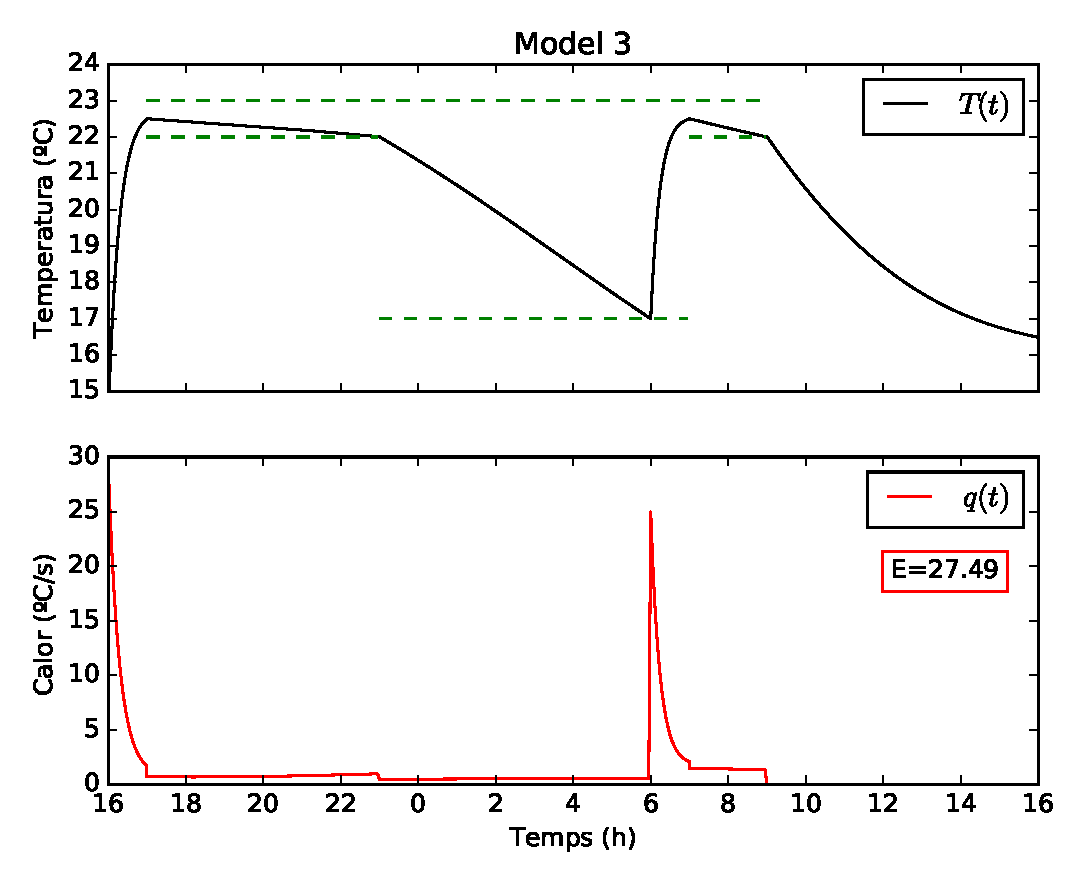
\includegraphics[width=12cm]{model3.eps}
	\caption{Evolució de la temperatura en l'habitatge i $q(t)$ aplicada. Les línies puntejades marquen el rang de temperatures que es considera acceptable en cada tram. Observem que aquest model es basa en poder regular el ritme al qual baixa la temperatura, per tant sempre cal que inicialment aquesta sigui superior a la que es considera mínima acceptable. El més eficient energèticament és fer que aquest mínim s'assoleixi al final de cada tram.}
	\label{figmodel3}
\end{figure}

Fer que la temperatura pugi fins a $22.5$ºC ha sigut una desició arbitrària, però observem que degut a la part de $q(t)$ que s'encarrega de pujar la temperatura, expressións \eqref{pujar1} i \eqref{pujar2}, augmentar aquesta fins a valors propers als $23$ºC és molt costós energèticament. 
\subsection*{Model 4}
Suposem ara que podem proporcionar una $q(t)$ infinita durant un temps infinitessimal $\delta t$, de manera que instantàniament es pot variar la temperatura una quantitat $\Delta T$. Es pot fer una estimació de la despesa energètica d'aquest model, ja que si integrem l'equació \eqref{principal}:
\begin{equation}
	\int_{T(t^*)}^{T(t^*+\delta t)}dT=\int_{t^*}^{t^*+\delta t}q(t)dt-k\int_{t^*}^{t^*+\delta t}(T-T_e)dt
\end{equation}
obtenim:
\begin{equation}
	E=\int_{t^*}^{t^*+\delta t}q(t)dt\leq \int_{T(t^*)}^{T(t^*+\delta t)}dT+kC\int_{t^*}^{t^*+\delta t}dt=\Delta T+kC\delta t
\end{equation}
on $C$ és una constant que compleix $|T-T_e|<C$. Com que $kC$ està fitat, i $\delta t$ és arbitrariament petit, tenim que $E\approx\Delta T$.  
\subsubsection*{Model 4.1}

\begin{figure}[h!]
	\centering
	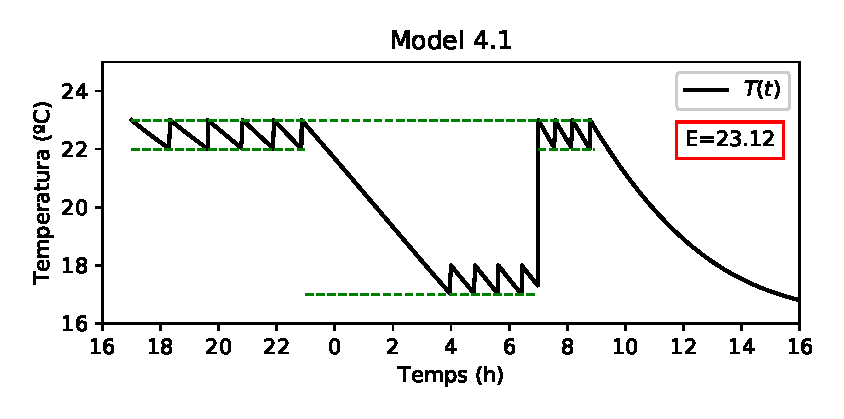
\includegraphics[width=13cm]{model41.eps}
\end{figure}
\subsubsection*{Model 4.2}
Mirem com podem optimitzar la despesa energètica si variem $\Delta T$
\begin{figure}[h!]
	\centering
	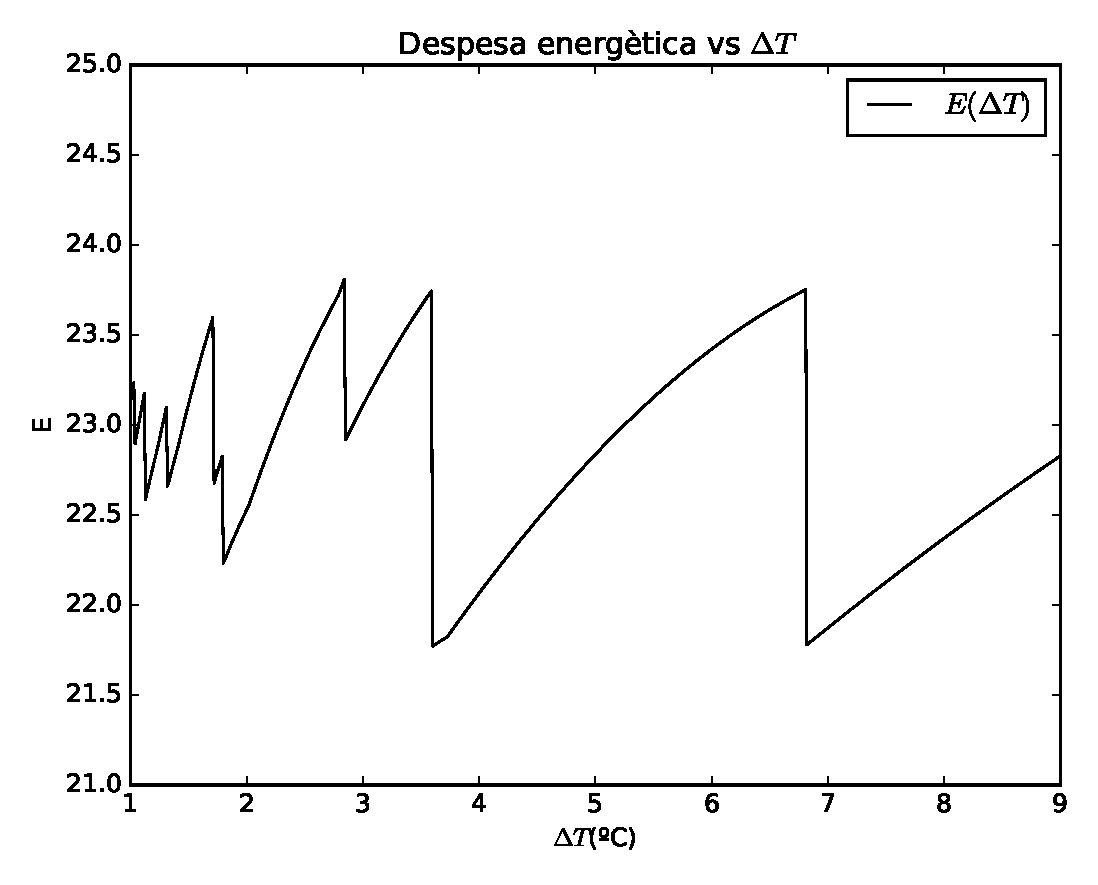
\includegraphics[width=13cm]{despesa.eps}
\end{figure}
\begin{figure}[h!]
	\centering
	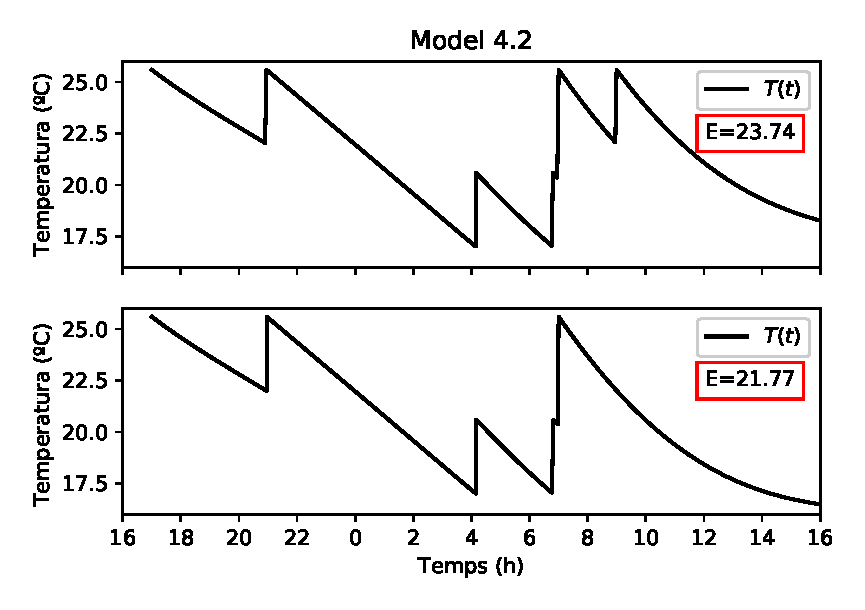
\includegraphics[width=13cm]{model42.eps}
\end{figure}
\section*{Conclusions}
\section*{Annex}
\end{document}